\documentclass[a4paper,12pt]{article}
\usepackage[T1]{fontenc}
\usepackage[utf8]{inputenc}
\usepackage{lmodern}
\usepackage[french]{babel}
\usepackage{url,csquotes}
\usepackage[hidelinks,hyperfootnotes=false]{hyperref}
\usepackage[titlepage]{polytechnique}
%\usepackage[titlepage,fancysections,pagenumber]{polytechnique}
\usepackage{float}
\usepackage{graphicx}
\usepackage{subfig}
\usepackage{tocloft}

\usepackage{tcolorbox}

\usepackage{titlesec}

% Define the font size for subsection headings
\titleformat{\subsubsection}
{\large\bfseries}{\thesubsubsection}{1em}{}

%\setcounter{tocdepth}{}
%\usepackage[charter]{mathdesign}

%\setcounter{secnumdepth}{0}


\title{Proposition détaillée}
\subtitle{Modélisation de la congestion portuaire à l’aide de GNN temporel}
\author{Isai Gordeev\\
Promotion X2022\\INF11}

\usepackage{hyperref}



\begin{document}

\maketitle

\section*{Résumé}

À écrire

\newpage


\tableofcontents

\newpage

\section{Les enjeux et la motivation du travail proposé}

Lorsque je suis arrivée en France, j'ai effectué un stage dans le sud de la France afin d'étudier le français de manière intensive et de m'immerger dans la culture et la formation préparatoire, de m'immerger dans l'environnement de l'École Polytechnique et dans ma culture scientifique en français et d'améliorer mon français afin de passer l'examen. C'était l'une des expériences les plus importantes, les plus intéressantes et les plus intenses de ma vie, au cours de laquelle j'ai beaucoup appris et je suis peut-être devenue une personne différente. Je détaille ci-dessous chaque activité, mes progrès et mes observations.

\section{La revue et une analyse de l’état de l’art ainsi que des approches concur- rentes et alternatives}

Avant mon arrivée en France, j'ai commencé à apprendre le français et à m'habituer à écrire en alphabet latin. J'ai lu un livre assez âgé avec des dialogues en français, ce qui m'a aidé à comprendre la France et la langue française, et qui m'a peut-être encore plus aidé pendant mon stage. Mais je n'ai pas du tout pratiqué la compréhension orale. À mon avis, apprendre le français consiste à apprendre deux langues différentes, le français oral et le français écrit, en raison du système syllabique de la langue, qui n'est pas évident pour les russophones. Le premier mois, malgré mon potentiel en grammaire et en vocabulaire, j'ai eu du mal à comprendre le français à l'oreille.


\section{Les objectifs intermédiaires et leur échéancier}


\section{L’organisation du travail et la répartition du travail }


\section{L'identification des moyens auxquels le projet fera appel, que ceux-ci soient mobilisables à l’École ou qu’ils soient à acheter}


\section{Les contributions des partenaires internes (laboratoires, binets) et externes (entreprises, organismes}


	
\section{Conclusion}

Dans ce rapport, j'ai décrit mon parcours et mon niveau de préparation, le déroulement de mes études à l'École Polytechnique avant le TC et mes projets pour l'avenir. J'ai essayé de couvrir autant que possible les différences culturelles, linguistiques et professionnelles que j'ai rencontrées pendant mon séjour en France et la manière dont je les ai plus ou moins bien gérées. C'était l'un des moments les plus inoubliables de ma vie et je suis sûr que ce ne sera pas le premier à l'École Polytechnique.  

En conclusion, je voudrais souligner une fois de plus ma forte motivation à réaliser mes projets et je voudrais remercier l'École Polytechnique, ses professeurs, ses employés, les organisateurs d'événements, l'atelier pour les opportunités qui m'ont été données.  

%\begin{figure}[htbp]
%	\centering
%	\begin{minipage}{0.3\textwidth}
%		\centering
%		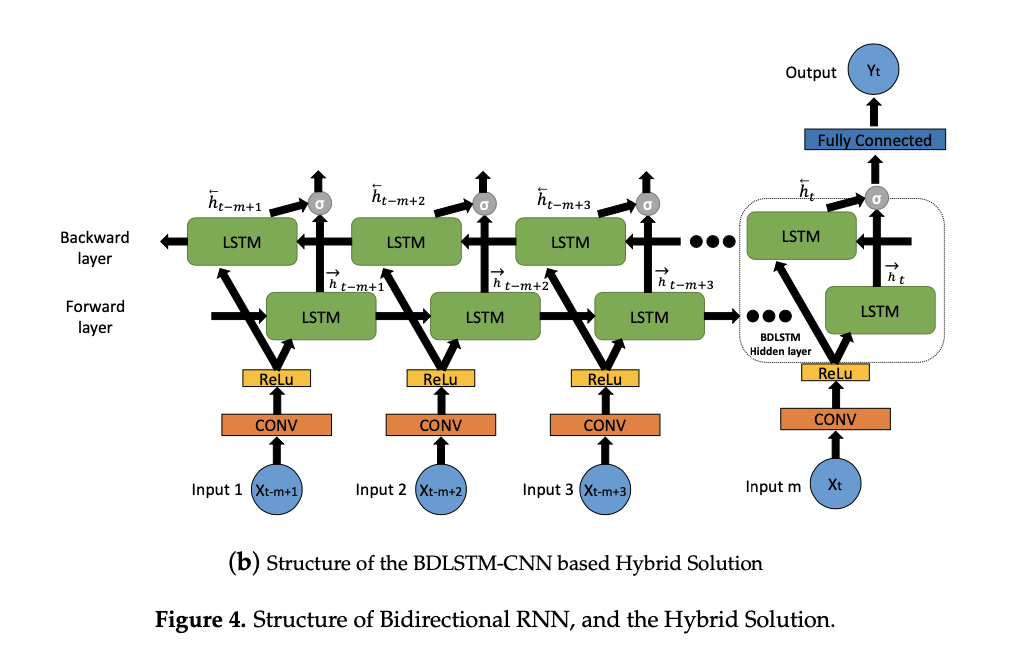
\includegraphics[width=\linewidth]{3}
%		\caption{Nos photos que Patrick a accrochées à son mur en souvenir de l'événement.}
%		\label{fig:image1}
%	\end{minipage}
%	\hfill
%	\begin{minipage}{0.3\textwidth}
%		\centering
%		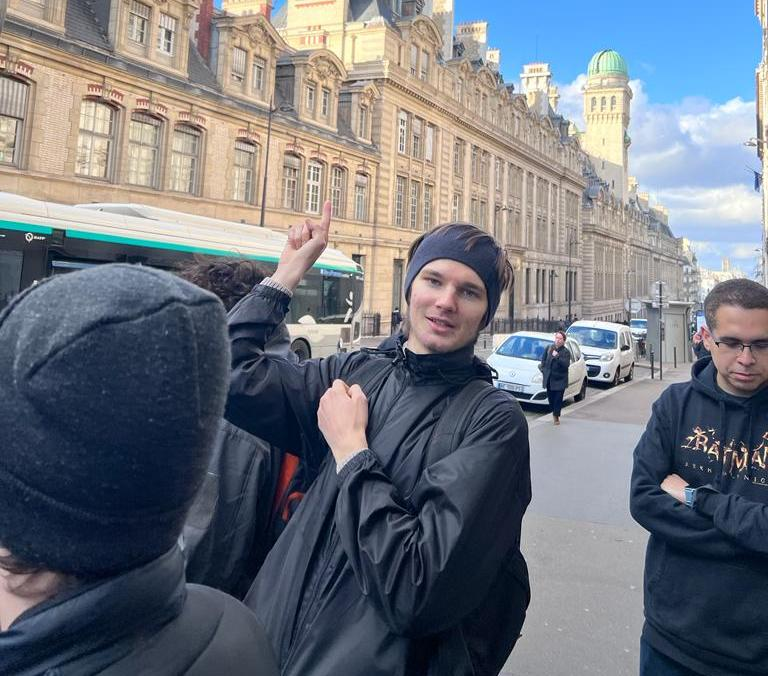
\includegraphics[width=\linewidth]{33}
%		\caption{Je montre le mur d'obus lors d'une randonnée dans le Quartier Latin}
%		\label{fig:image2}
%	\end{minipage}
%	\hfill
%	\begin{minipage}{0.3\textwidth}
%		\centering
%		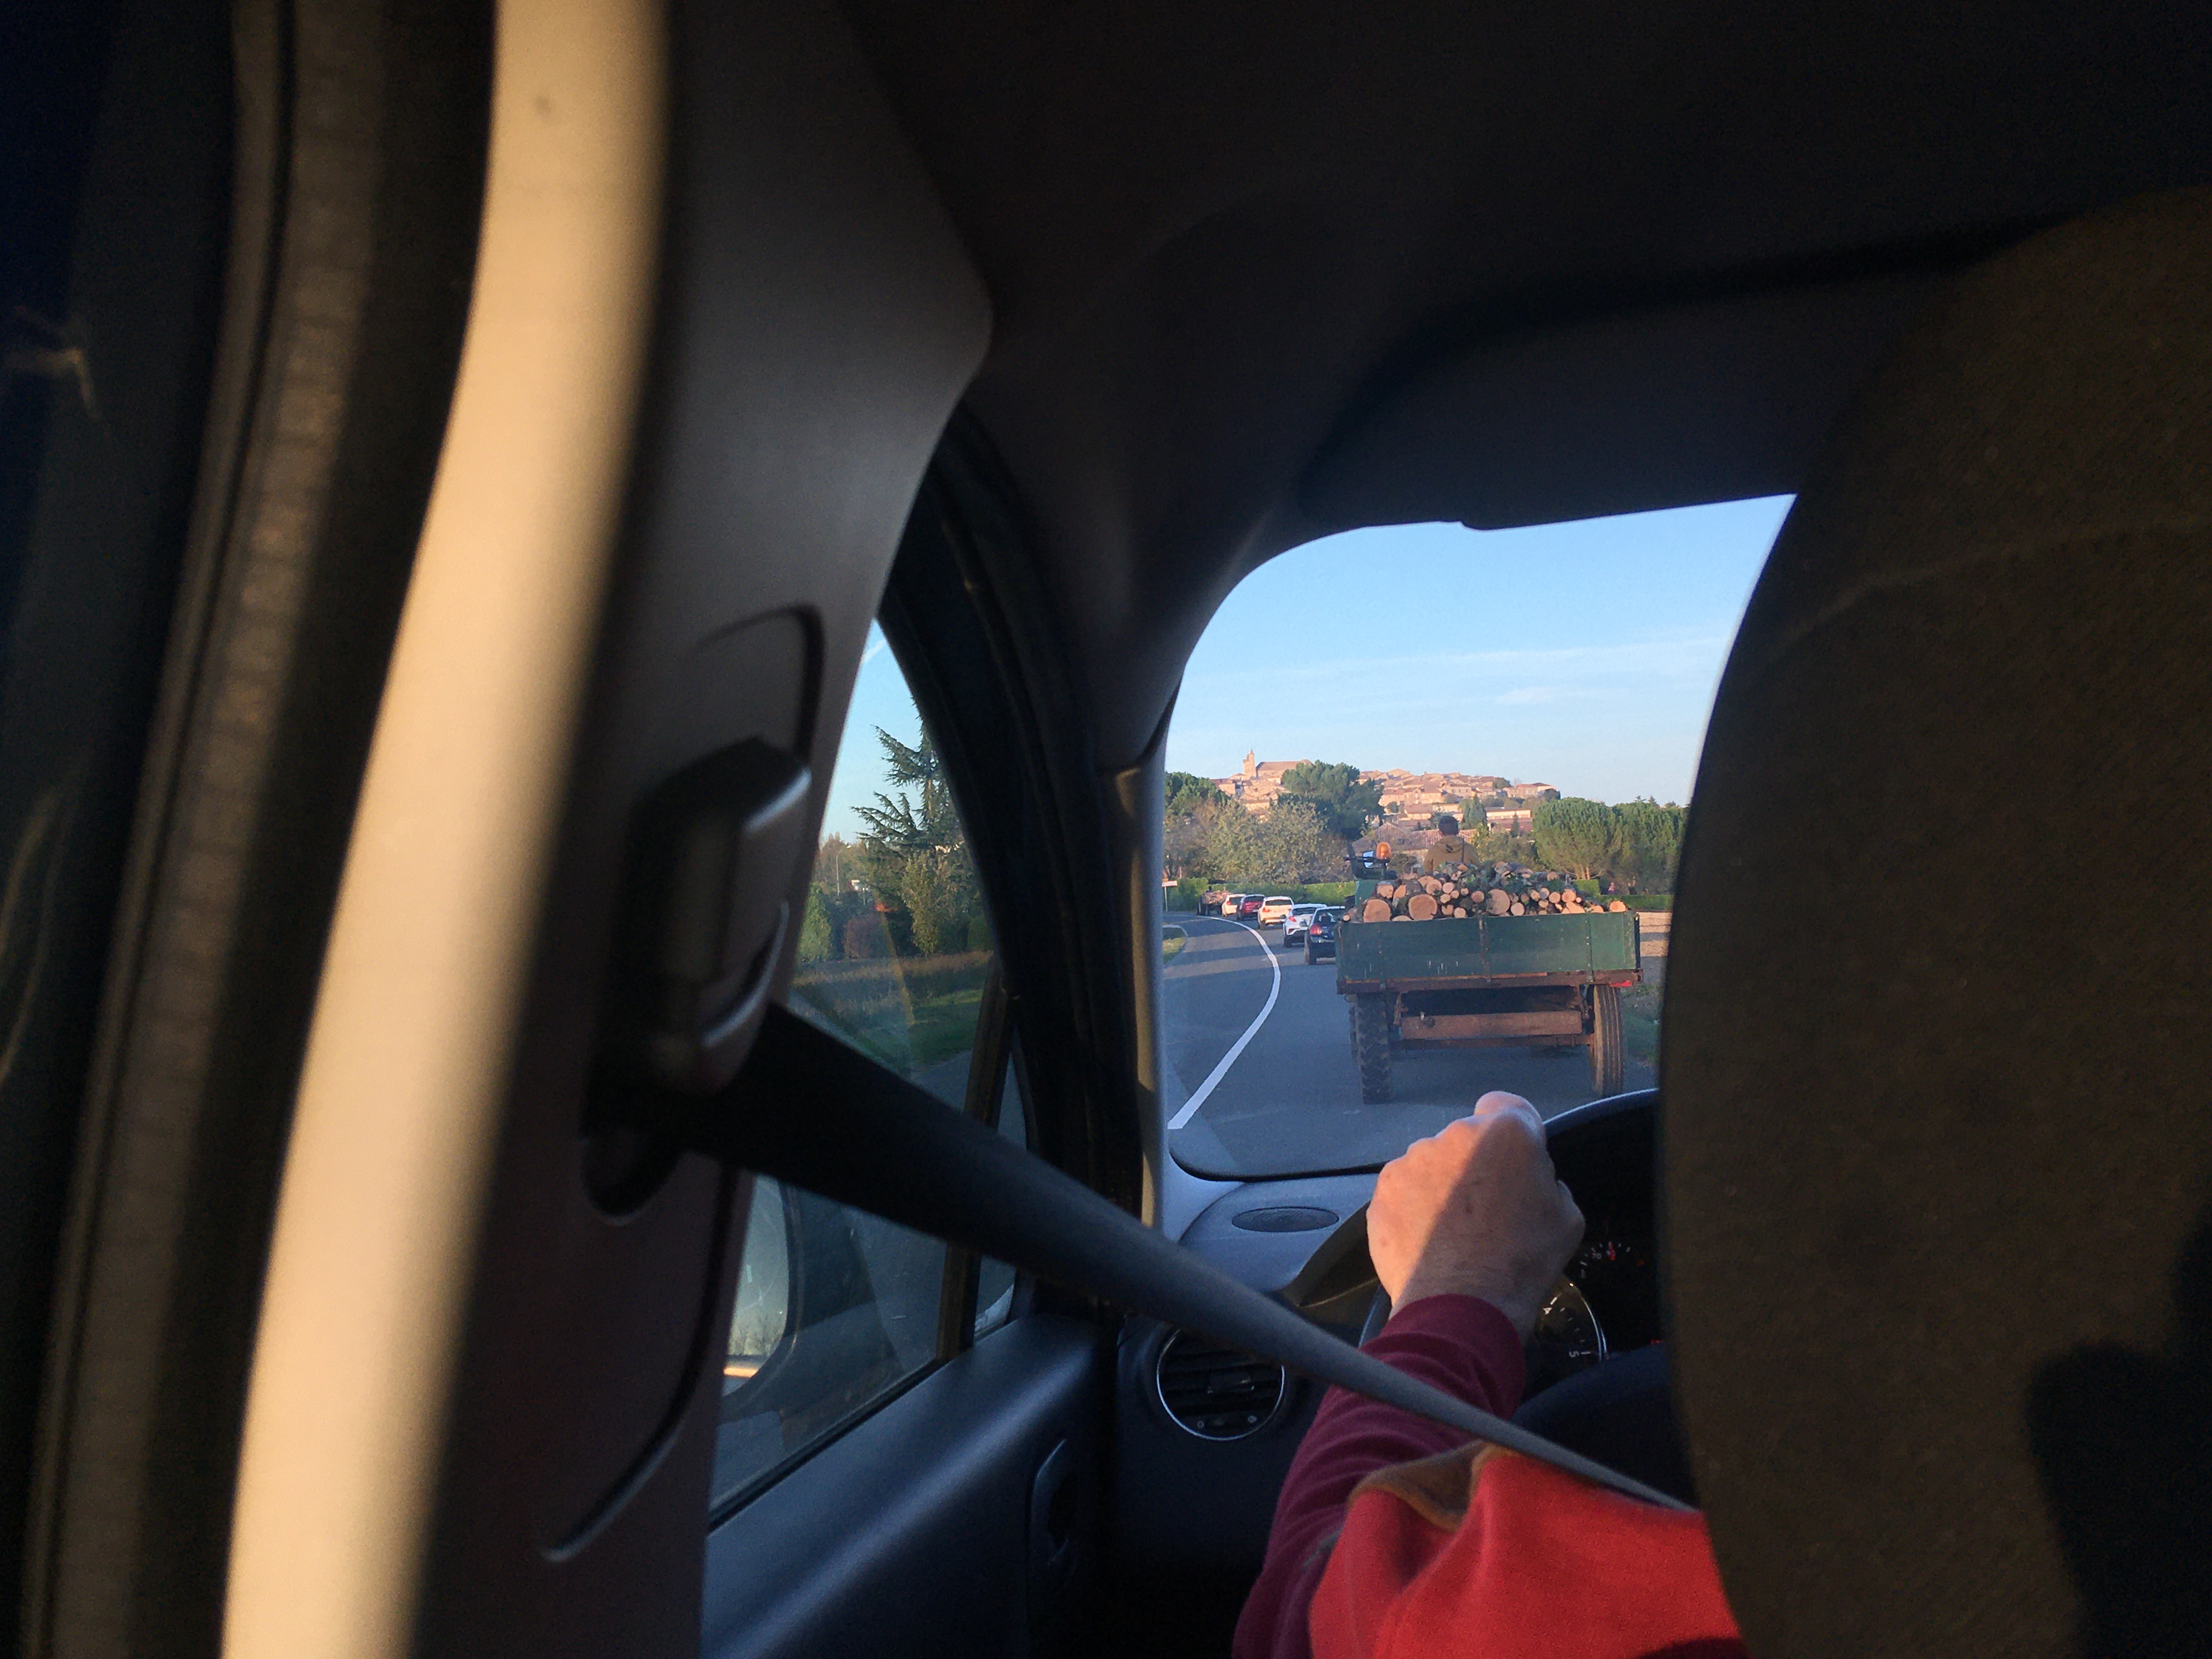
\includegraphics[width=\linewidth]{321}
%		\caption{Patrick nous emmène dans un village vieux de 1000 ans.}
%		\label{fig:image3}
%	\end{minipage}
%	\label{fig:myfigure}
%\end{figure}
%
%\begin{figure}[htbp]
%	\centering
%	\begin{minipage}{0.3\textwidth}
%		\centering
%		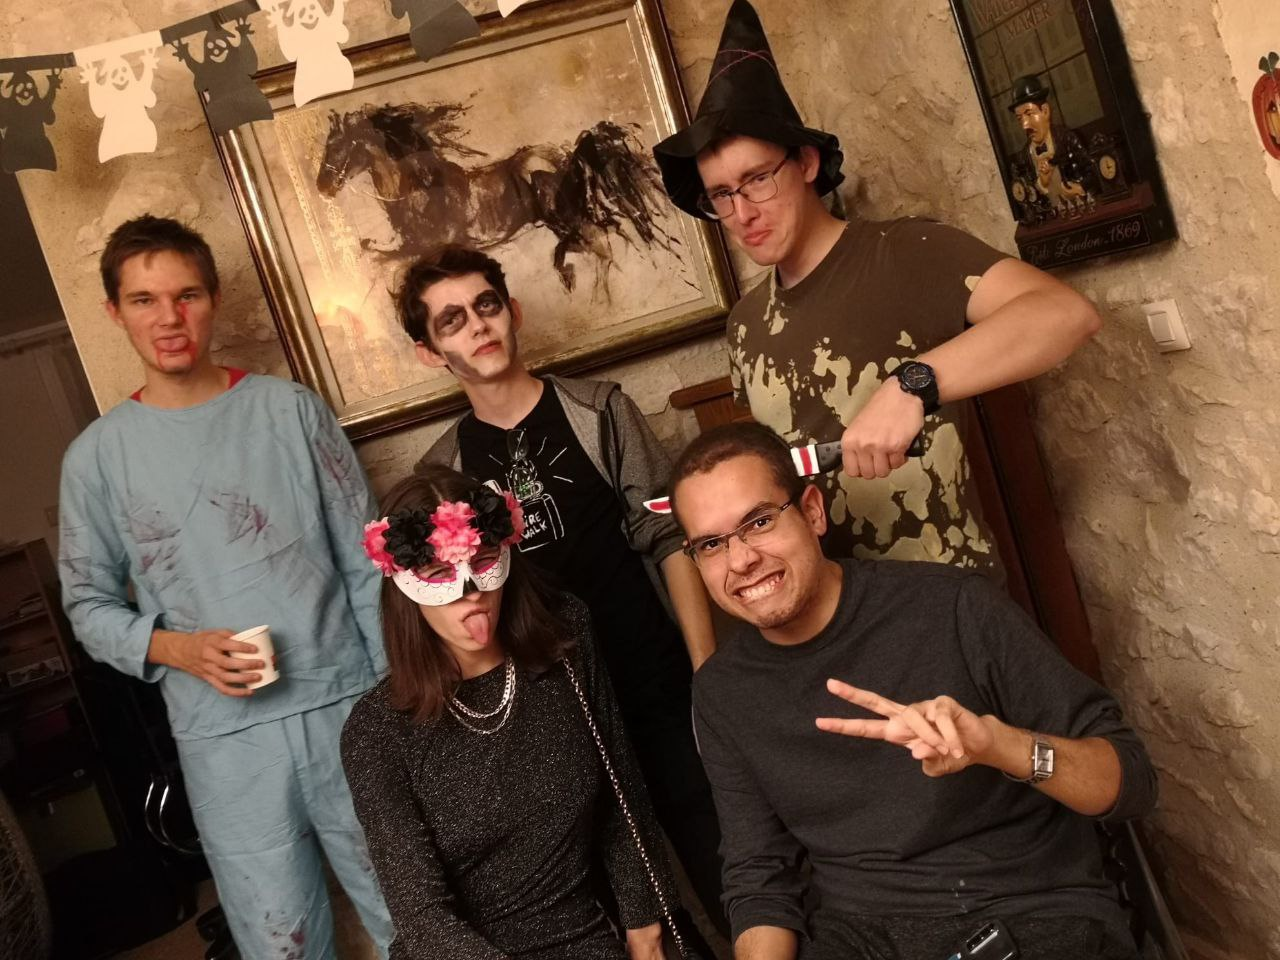
\includegraphics[width=\linewidth]{4}
%		\caption{À l'occasion de Halloween dans la famille d'accueil de mon ami}
%		\label{fig:image1}
%	\end{minipage}
%	\hfill
%	\begin{minipage}{0.3\textwidth}
%		\centering
%		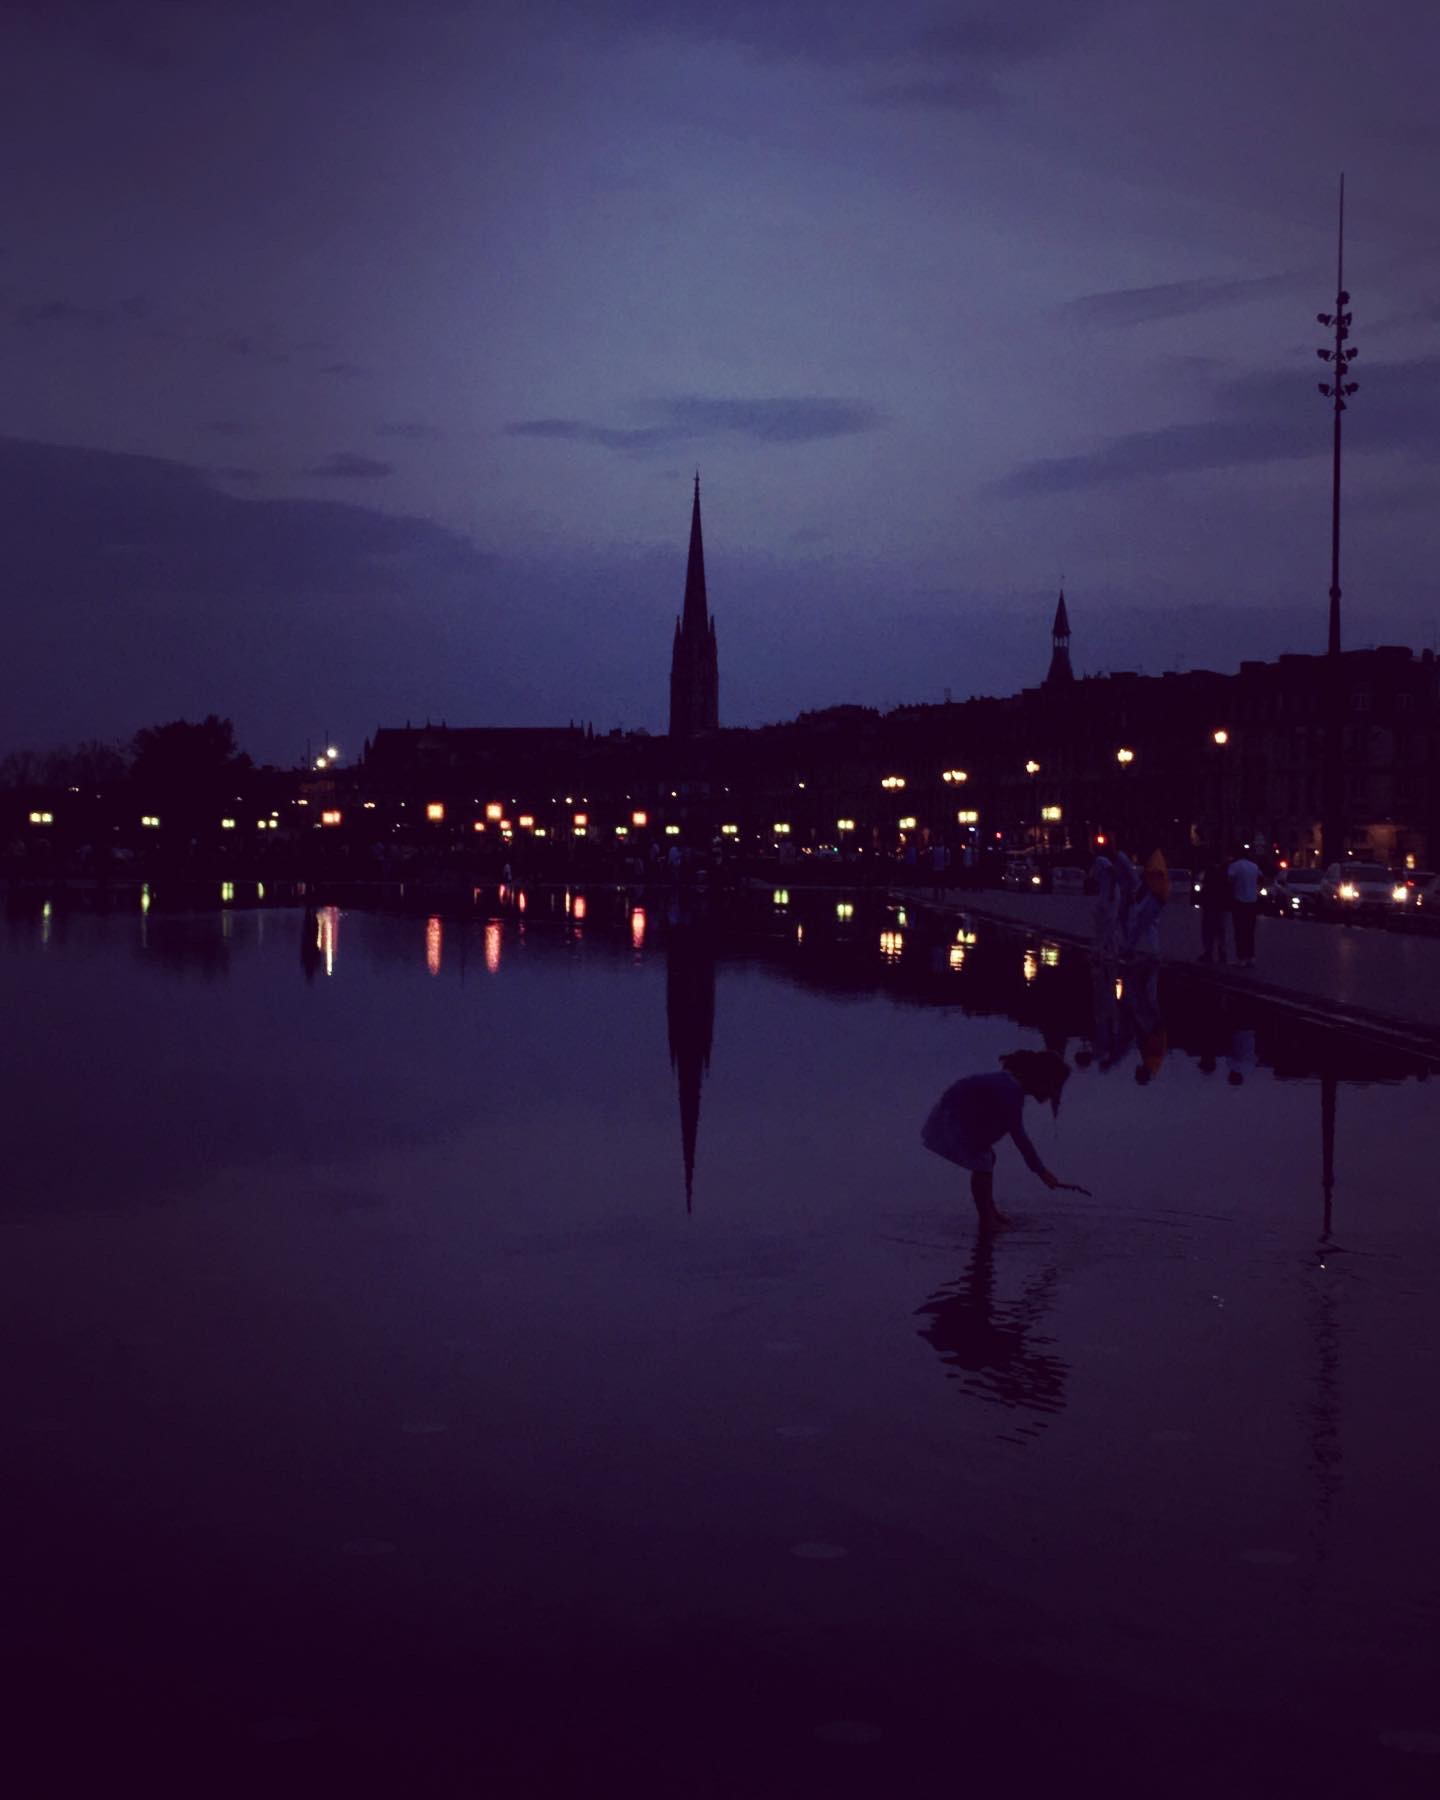
\includegraphics[width=\linewidth]{43}
%		\caption{La photo prise à Bordeaux lors d'un week-end à Villeneuve}
%		\label{fig:image2}
%	\end{minipage}
%	\hfill
%	\begin{minipage}{0.3\textwidth}
%		\centering
%		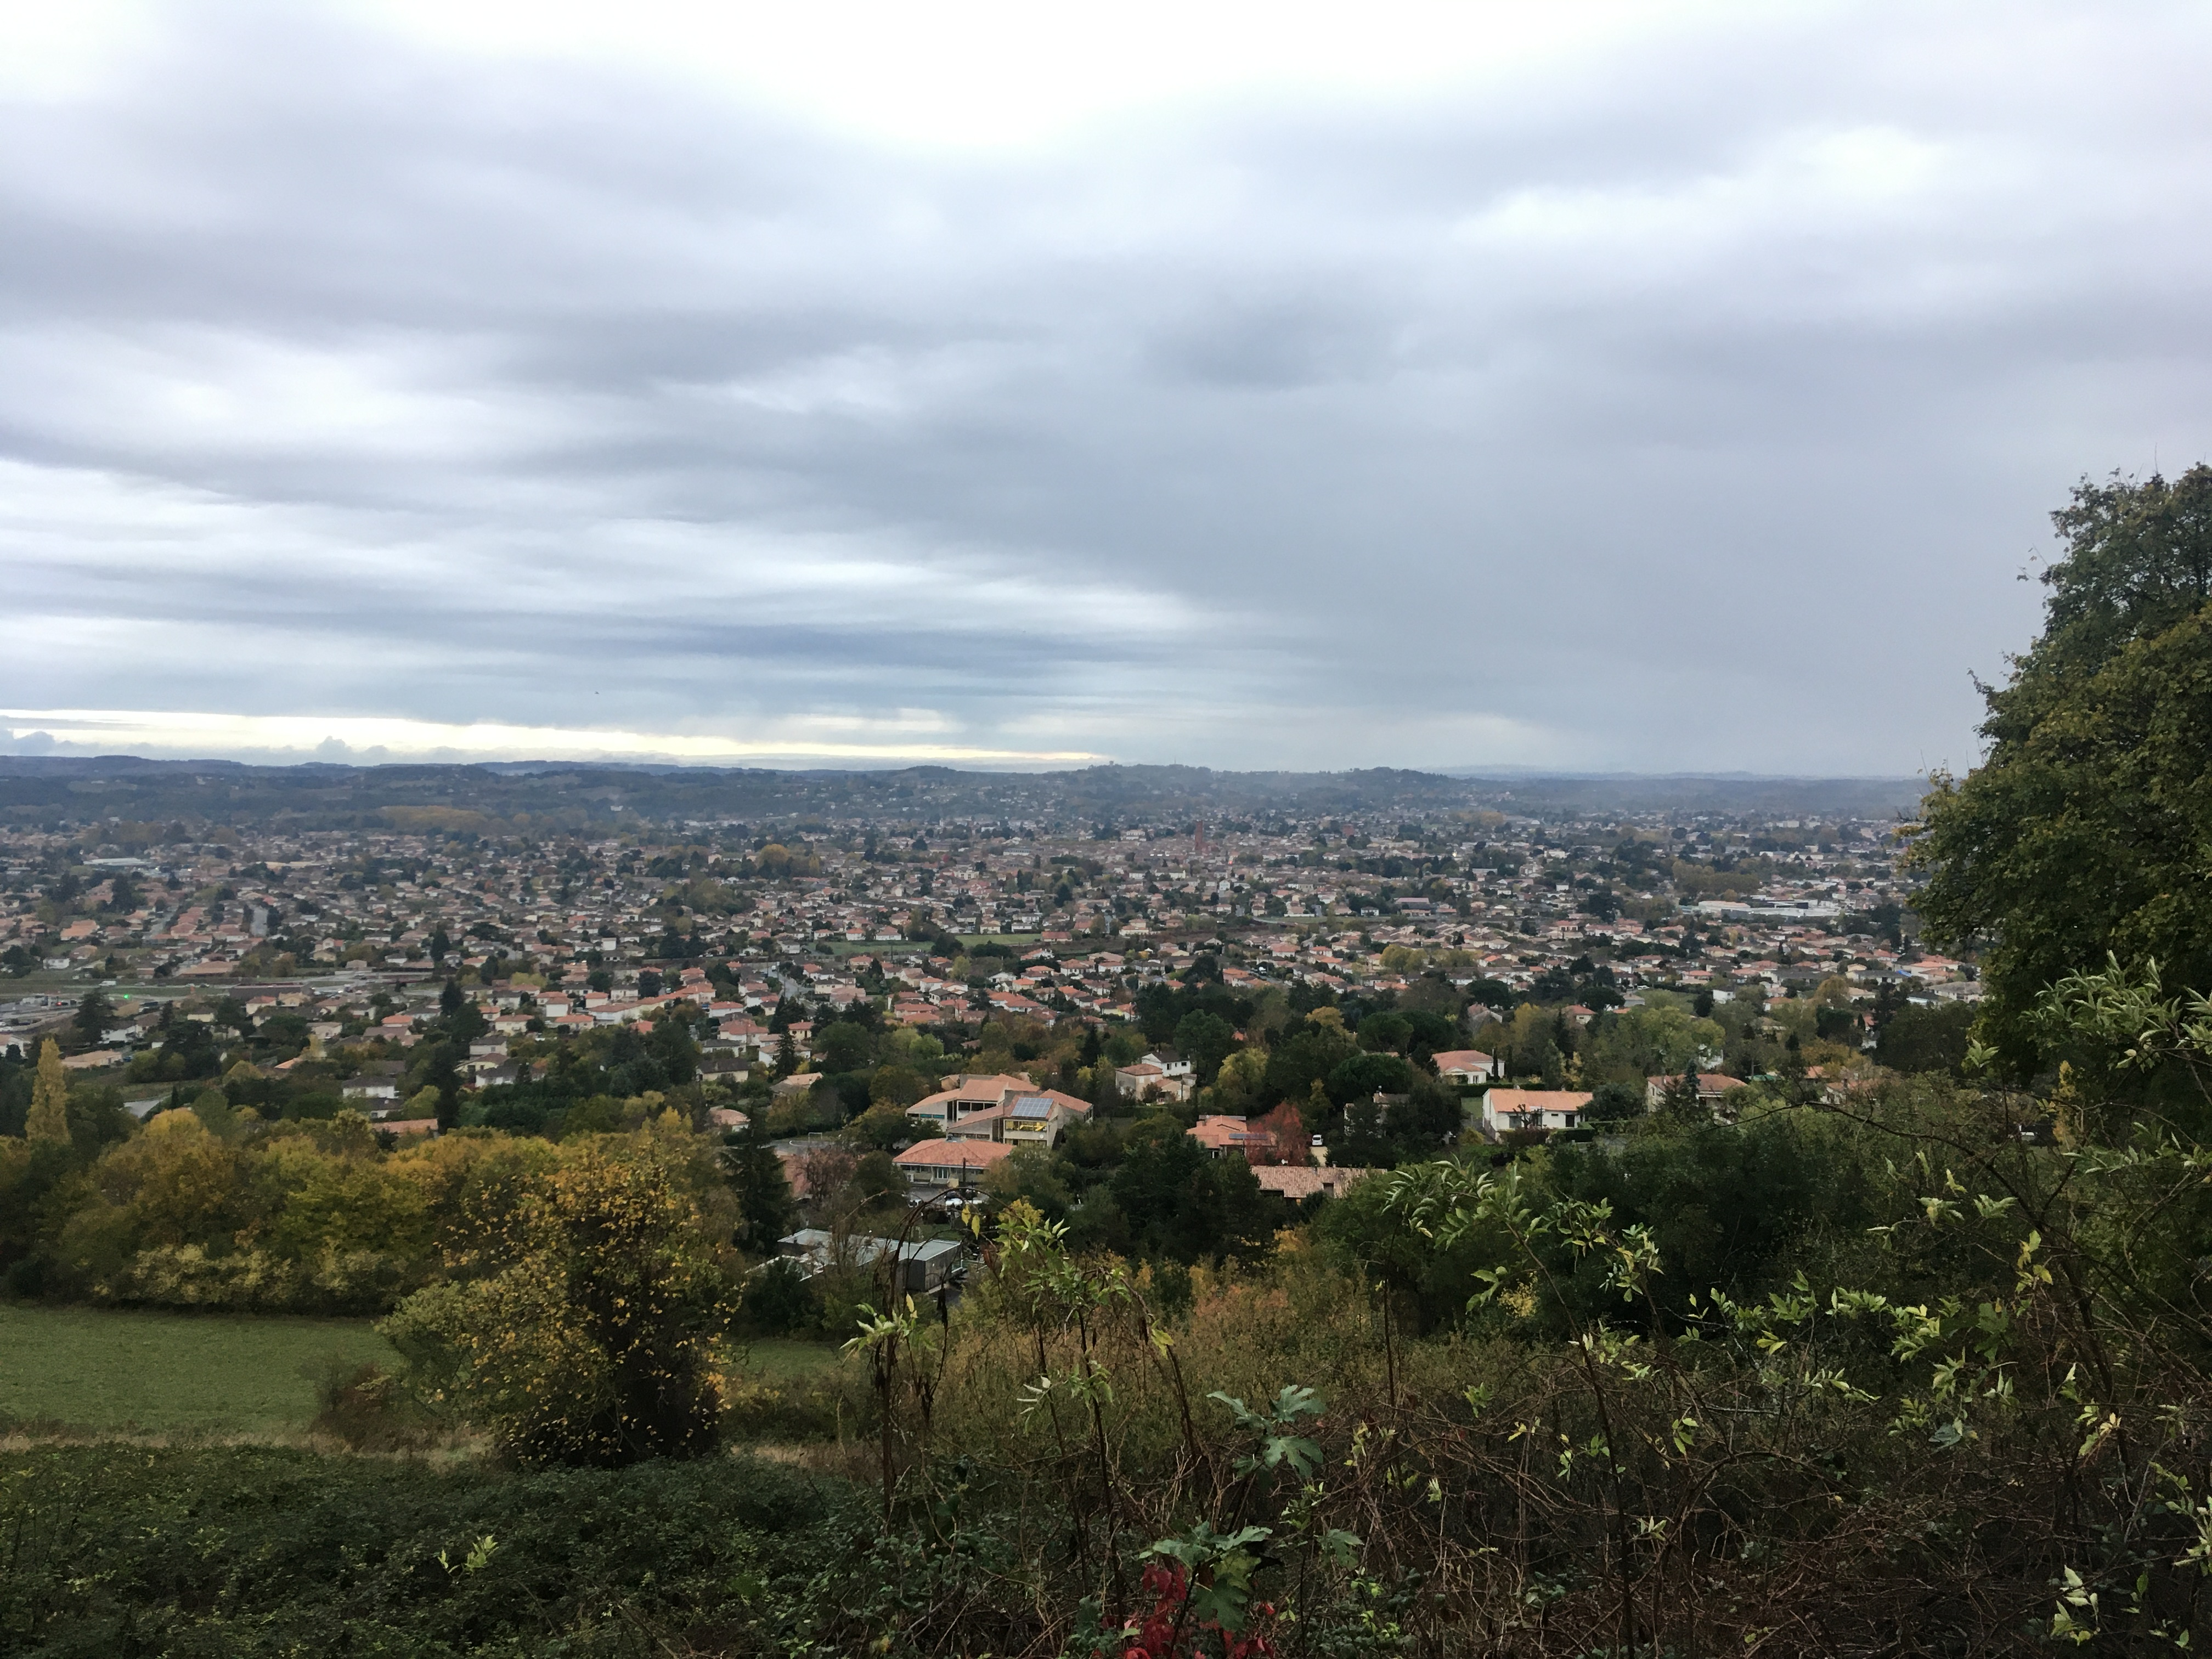
\includegraphics[width=\linewidth]{123}
%		\caption{Une photo de Villeneuve que j'ai prise lors de ma promenade}
%		\label{fig:image3}
%	\end{minipage}
%	\label{fig:myfigure}
%\end{figure}

\end{document}